\documentclass[a4paper,11pt]{article}

\usepackage[utf8]{inputenc}
\usepackage[T1]{fontenc}
\usepackage{lmodern}
\usepackage{amsmath, amssymb}
\usepackage{graphicx}
\usepackage{booktabs}
\usepackage{xcolor}
\usepackage{algorithm}
\usepackage{algpseudocode}
\usepackage{hyperref}
\usepackage{geometry}
\geometry{margin=2.4cm}
\hypersetup{
    colorlinks=true,
    linkcolor=blue!50!black,
    citecolor=blue!50!black,
    urlcolor=blue!60!black
}

\graphicspath{{../outputs/2026-05-11_dr-comparison/}}

\title{%
    Comparing two dead-reckoning methods on smart-ring brushing data:\\
    the in-house heuristic versus a faithful port of AEOLUS \cite{radeta2023}%
}
\author{%
    Qun Yan Li\\
    \small University of Tartu --- Pervasive Data Science Seminar\\
    \small \texttt{li\_qun\_yan@outlook.com}%
}
\date{11 May 2026}

\begin{document}
\maketitle

\begin{abstract}
The \texttt{ringbrush-coverage} project visualises toothbrushing coverage from
smart-ring inertial logs. A small dead-reckoning (DR) step inside the analysis
pipeline nudges the brush cursor in response to short-term motion. The
production pipeline ships with an in-house \emph{heuristic} integrator. In this
note we add a faithful port of the AEOLUS dead-reckoning pipeline described in
Sections~3.3--3.6 of Radeta et al.\ \cite{radeta2023}, and compare the two
methods on four labelled sessions. The heuristic captures repetitive
oscillation cleanly but yields non-metric output. AEOLUS produces metric
trajectories but collapses to near-1D drift on short, repetitive brushing
clips because the brush almost never crosses the paper's
zero-velocity-update (ZVU) threshold. On full-session data, both methods
recover a similarly-structured path. We discuss the convention assumptions
and tuning choices that shape this comparison.
\end{abstract}

\section{Background}

The \texttt{ringbrush-coverage} pipeline parses smart-ring CSV logs of the form
$\langle t_{ms}, \mathrm{roll}, \mathrm{pitch}, \mathrm{yaw}, a_x, a_y, a_z
\rangle$, classifies each analysis window into one of six mouth-region labels,
and accumulates per-zone coverage seconds. A short per-window dead-reckoning
pass computes a tiny displacement $(\Delta x, \Delta y)$ that perturbs the
classifier's anchor cursor so the rendered brush tip jitters in the direction
the user is actually moving. The DR result is small by design: it is a visual
aid, not a metric trajectory.

Radeta et al.\ \cite{radeta2023} systematically evaluate fifteen dead-reckoning
algorithms in underwater and ground environments using their AEOLUS apparatus
(an MPU-9250 IMU on a LoPy4). Their pipeline is built around the
sensor-fusion-then-double-integration recipe: orientation estimation
(Madgwick by default), Earth-frame gravity removal, double integration with a
ZVU-style drift reduction step, and a final heading-projected position
update.

\section{The two methods}

We use the following notation. At each time step $i$, the IMU reports Euler
angles $(\phi_i, \theta_i, \psi_i) = (\mathrm{roll}_i, \mathrm{pitch}_i,
\mathrm{yaw}_i)$ in degrees and a body-frame acceleration vector
$\mathbf{a}_i = (a_{x,i}, a_{y,i}, a_{z,i})$ in m/s$^2$. The time step is
$\Delta t_i = (t_i - t_{i-1})/1000$\,s.

\subsection{Heuristic DR (existing implementation)}

The shipping implementation in
\href{../ringbrush_coverage/core.py}{\texttt{ringbrush\_coverage/core.py}}
treats the per-window mean of the in-plane accelerometer as a gravity proxy
and feeds the residual through a damped integrator, with two small attitude
terms that nudge the position by yaw and pitch differences. Concretely, for
each window of samples $\{(\mathbf{a}_i, \phi_i, \theta_i, \psi_i)\}_{i=0}^{N-1}$:

\begin{algorithm}[H]
\caption{Heuristic dead reckoning (per window).}
\label{alg:heuristic}
\begin{algorithmic}[1]
\State $\bar a_x \gets \mathrm{mean}\{a_{x,i}\}, \quad \bar a_y \gets \mathrm{mean}\{a_{y,i}\}$
\State $v_x, v_y, p_x, p_y \gets 0$
\For{$i = 1, \dots, N-1$}
    \State $\delta a_x \gets a_{x,i} - \bar a_x; \quad \delta a_y \gets a_{y,i} - \bar a_y$
    \State $v_x \gets 0.92 \cdot v_x + 2.00 \cdot \delta a_x \cdot \Delta t_i$
    \State $v_y \gets 0.92 \cdot v_y - 2.00 \cdot \delta a_y \cdot \Delta t_i$
    \State $p_x \gets p_x + v_x \cdot \Delta t_i + 0.0015 \cdot \mathrm{circDelta}(\psi_i, \psi_{i-1})$
    \State $p_y \gets p_y + v_y \cdot \Delta t_i$
\EndFor
\State \Return $(p_x, p_y)$
\end{algorithmic}
\end{algorithm}

The four constants ($0.92$ damping, $2.00$ acceleration scale, $0.0015$ yaw
contribution, and $0$ pitch contribution) were grid-searched against three
labelled motion sessions (up-down, left-right, inside-outside) so that the
P90 of $|p_x|$ and $|p_y|$ matched design targets in the cursor's normalised
visualisation space ($[0, 1] \times [0, 1]$). The output is therefore unitless;
it lives directly in viz coordinates.

\subsection{AEOLUS DR (faithful port of Radeta 2023)}

AEOLUS performs gravity removal via the device orientation, then integrates
twice with a ZVU step, then applies a heading projection. The port in
\href{../ringbrush_coverage/core.py}{\texttt{core.py}} skips the Madgwick
fusion stage because the ring already emits Euler angles directly. We assume
the device's roll and pitch follow the ZYX intrinsic Tait-Bryan convention
with world $+z$ up; under that convention, the expected gravity vector in
body frame is
\begin{equation}
\mathbf{g}_b(\phi, \theta) = g \begin{pmatrix} -\sin\theta \\ \cos\theta\sin\phi \\ \cos\theta\cos\phi \end{pmatrix},
\qquad g = 9.81\,\mathrm{m/s^2}.
\label{eq:gravity}
\end{equation}
The linear acceleration is $\mathbf{a}_{\mathrm{lin},i} = \mathbf{a}_i -
\mathbf{g}_b(\phi_i, \theta_i)$.

The drift reduction (Algorithm~\ref{alg:aeolus-zvu}) is transcribed
\emph{verbatim} from \cite[Algorithm~1]{radeta2023}: when the linear
acceleration along an axis is near zero the velocity is decayed, otherwise
the velocity is \emph{replaced} (not accumulated) with $a \cdot \Delta t$.
This replacement reading is almost certainly a typesetting error in the
paper, but we follow the letter rather than the spirit of the text here. We
return to this point in Section~\ref{sec:discussion}.

\begin{algorithm}[H]
\caption{AEOLUS drift reduction \cite[Algorithm 1]{radeta2023}, applied per axis.}
\label{alg:aeolus-zvu}
\begin{algorithmic}[1]
\If{$|a| < \varepsilon$} \Comment{$\varepsilon = 0.05$\,m/s$^2$}
    \State $v \gets v \cdot \beta$ \Comment{$\beta = 0.55$ for $x,y$; $0.80$ for $z$}
\Else
    \State $v \gets a \cdot \Delta t$ \Comment{verbatim from the paper}
\EndIf
\end{algorithmic}
\end{algorithm}

The position update follows equation 9 of the paper, projecting the body-frame
step through the heading angle $\psi_i$:
\begin{equation}
\begin{aligned}
p_{x,i} &= \Delta x_i \cdot \cos\psi_i + p_{x,i-1}, \\
p_{y,i} &= \Delta y_i \cdot \sin\psi_i + p_{y,i-1},
\end{aligned}
\qquad
\Delta x_i = v_x \cdot \Delta t_i,\ \Delta y_i = v_y \cdot \Delta t_i.
\label{eq:eq9}
\end{equation}

The output is in metres. For the cursor placement inside
\texttt{analyze\_session}, we rescale per session so the P90 of $|\Delta x|$
and $|\Delta y|$ matches the heuristic's design target ($\approx 0.35$ viz
units). The comparison tool plots the raw, un-rescaled metric trajectory.

\section{Implementation in the codebase}

The faithful port is in
\href{../ringbrush_coverage/core.py}{\texttt{ringbrush\_coverage/core.py}} as
the function \texttt{estimate\_dead\_reckoning\_aeolus}, alongside session-wide
helpers \texttt{trajectory\_heuristic} and \texttt{trajectory\_aeolus} that emit
one point per sensor reading. A new CLI flag
\texttt{--dr-method \{heuristic,aeolus\}} selects the method end-to-end. The
session-wide trajectory generators back a dedicated comparison driver at
\href{../tools/compare_dead_reckoning.py}{\texttt{tools/compare\_dead\_reckoning.py}},
which writes a JSON stats summary, a static PNG, and an animated MP4 per input
log. The new functions are exercised by five unit tests in
\href{../tests/test_core.py}{\texttt{tests/test\_core.py}} (stationary input,
empty input, trajectory length consistency, body-x response, and
\texttt{analyze\_session(dr\_method="aeolus")} integration), all passing
together with the four pre-existing tests.

\section{Experimental setup}

We ran the comparison driver on four sessions:

\begin{itemize}
    \item \texttt{left-and-right-and-...} (10\,s, labelled lateral motion).
    \item \texttt{up-and-down-and-...} (29\,s, labelled vertical motion).
    \item \texttt{inside-and-outside-and-...} (35\,s, labelled in-out motion).
    \item \texttt{full-session} (62\,s, freeform full brushing).
\end{itemize}

For each session, both methods run once on the full sample stream (no
windowing, no per-window resets) and accumulate a continuous 2D trajectory.
Per-method summary statistics include the cumulative path length, the
end-to-start displacement, and the bounding-box diagonal of the path.

\section{Results}
\label{sec:results}

Table~\ref{tab:summary} reports the per-session stats. Path length and bounding
box are reported in each method's native unit (the heuristic in normalised viz
units, AEOLUS in metres); the path/end ratio expresses how much of a method's
travel \emph{cancels} when integrated --- low values mean lots of oscillation
back to the origin, high values mean a drift-dominated path.

\begin{table}[h]
\centering
\caption{Per-session DR statistics. ``path/end'' is end-displacement divided
by total path length; lower is more oscillatory, higher is more
drift-dominated.}
\label{tab:summary}
\begin{tabular}{lrrrrrr}
\toprule
& \multicolumn{3}{c}{Heuristic (viz units)} & \multicolumn{3}{c}{AEOLUS (metres)} \\
\cmidrule(lr){2-4}\cmidrule(lr){5-7}
Session            & path  & bbox  & end/path & path  & bbox  & end/path \\
\midrule
left-right         &  23.7 &  3.82 & 0.009 &  1.63 & 1.21 & 0.73 \\
up-down            &  30.2 &  2.97 & 0.007 &  1.55 & 1.34 & 0.86 \\
inside-outside     &  14.7 &  2.77 & 0.007 &  3.35 & 3.33 & 0.99 \\
full-session       & 109.7 & 42.79 & 0.015 &  7.11 & 3.73 & 0.47 \\
\bottomrule
\end{tabular}
\end{table}

The qualitative shape of each session is shown in
Figures~\ref{fig:lr}--\ref{fig:full}. Each panel uses independent, data-fit
axes, so the shapes are directly comparable but the magnitudes are not.

\begin{figure}[h]
\centering
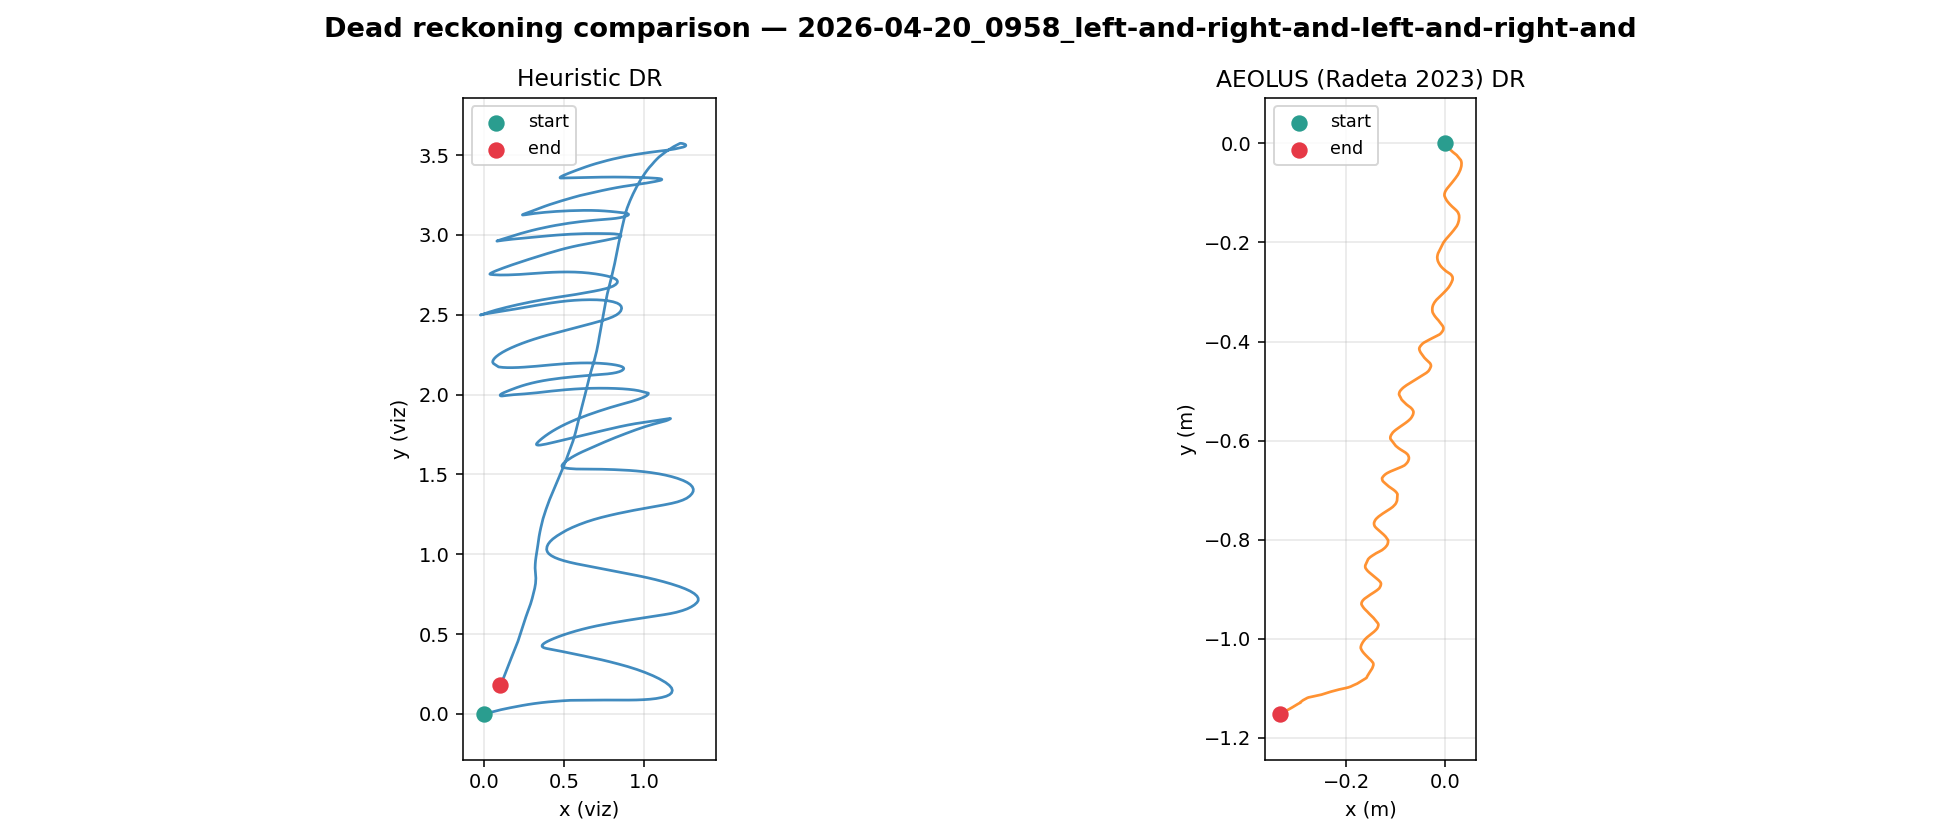
\includegraphics[width=\linewidth]{2026-04-20_0958_left-and-right-and-left-and-right-and_dr-compare.png}
\caption{Lateral brushing session. The heuristic (left) cleanly captures the
left-right oscillation; AEOLUS (right) drifts roughly south-southwest with
small ripples on top.}
\label{fig:lr}
\end{figure}

\begin{figure}[h]
\centering
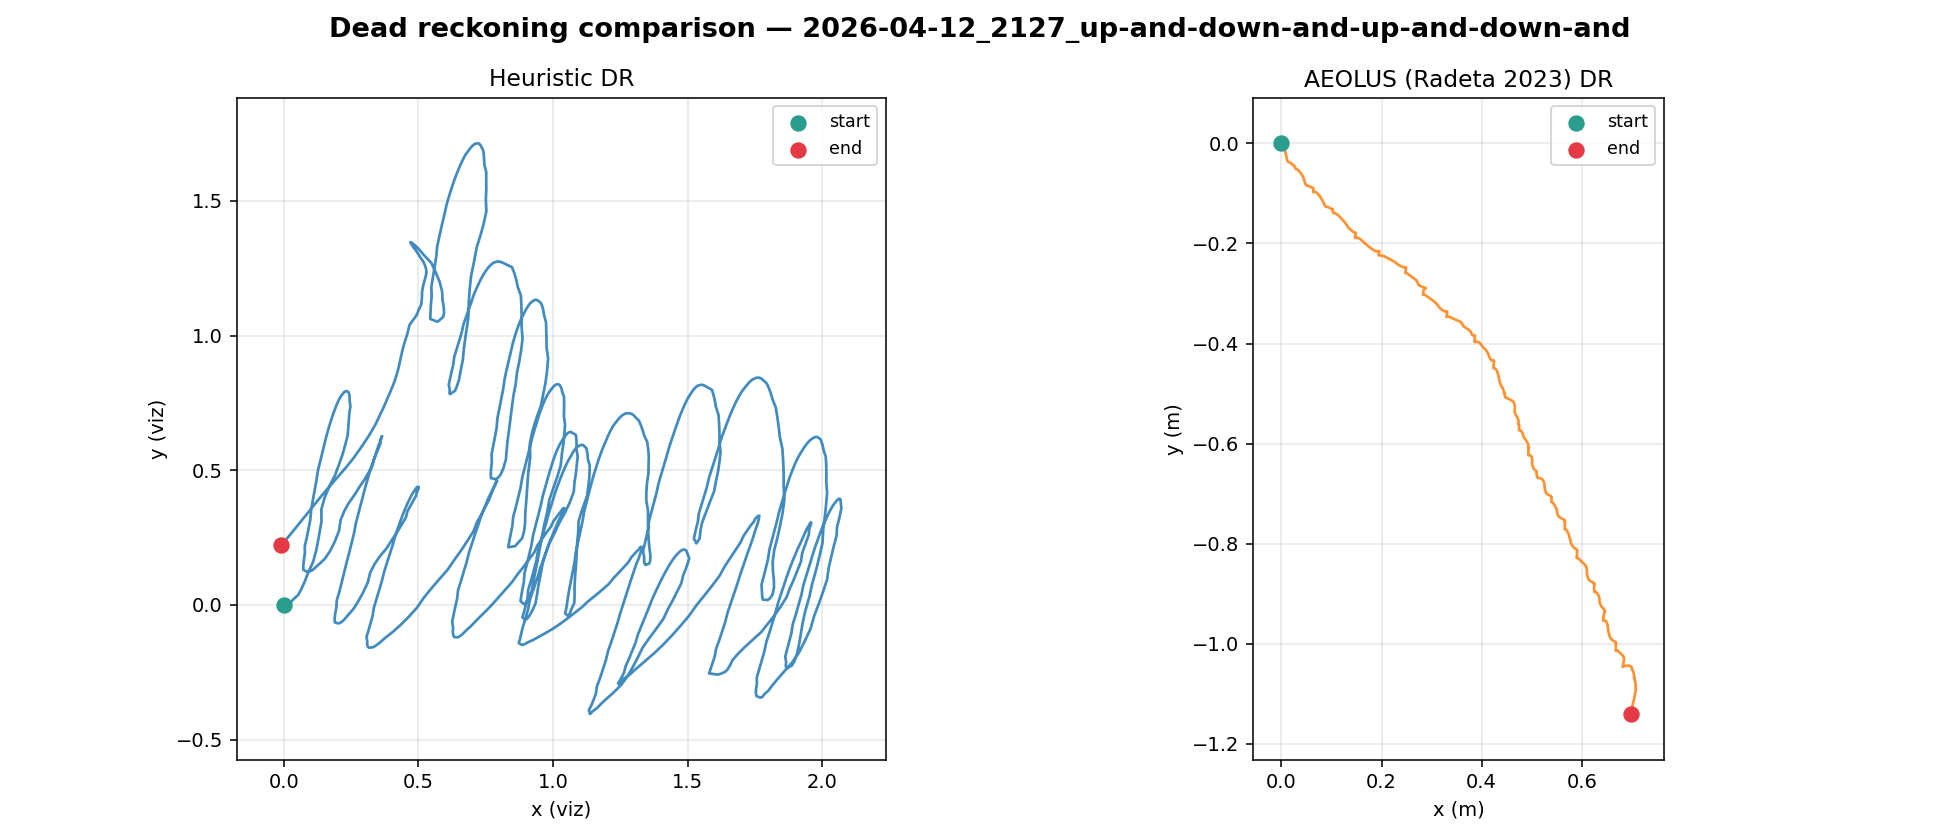
\includegraphics[width=\linewidth]{2026-04-12_2127_up-and-down-and-up-and-down-and_dr-compare.png}
\caption{Vertical brushing session. The heuristic produces a recognisable
``saw-tooth'' fan of strokes; AEOLUS reduces this to a smooth drift toward
the lower right.}
\label{fig:ud}
\end{figure}

\begin{figure}[h]
\centering
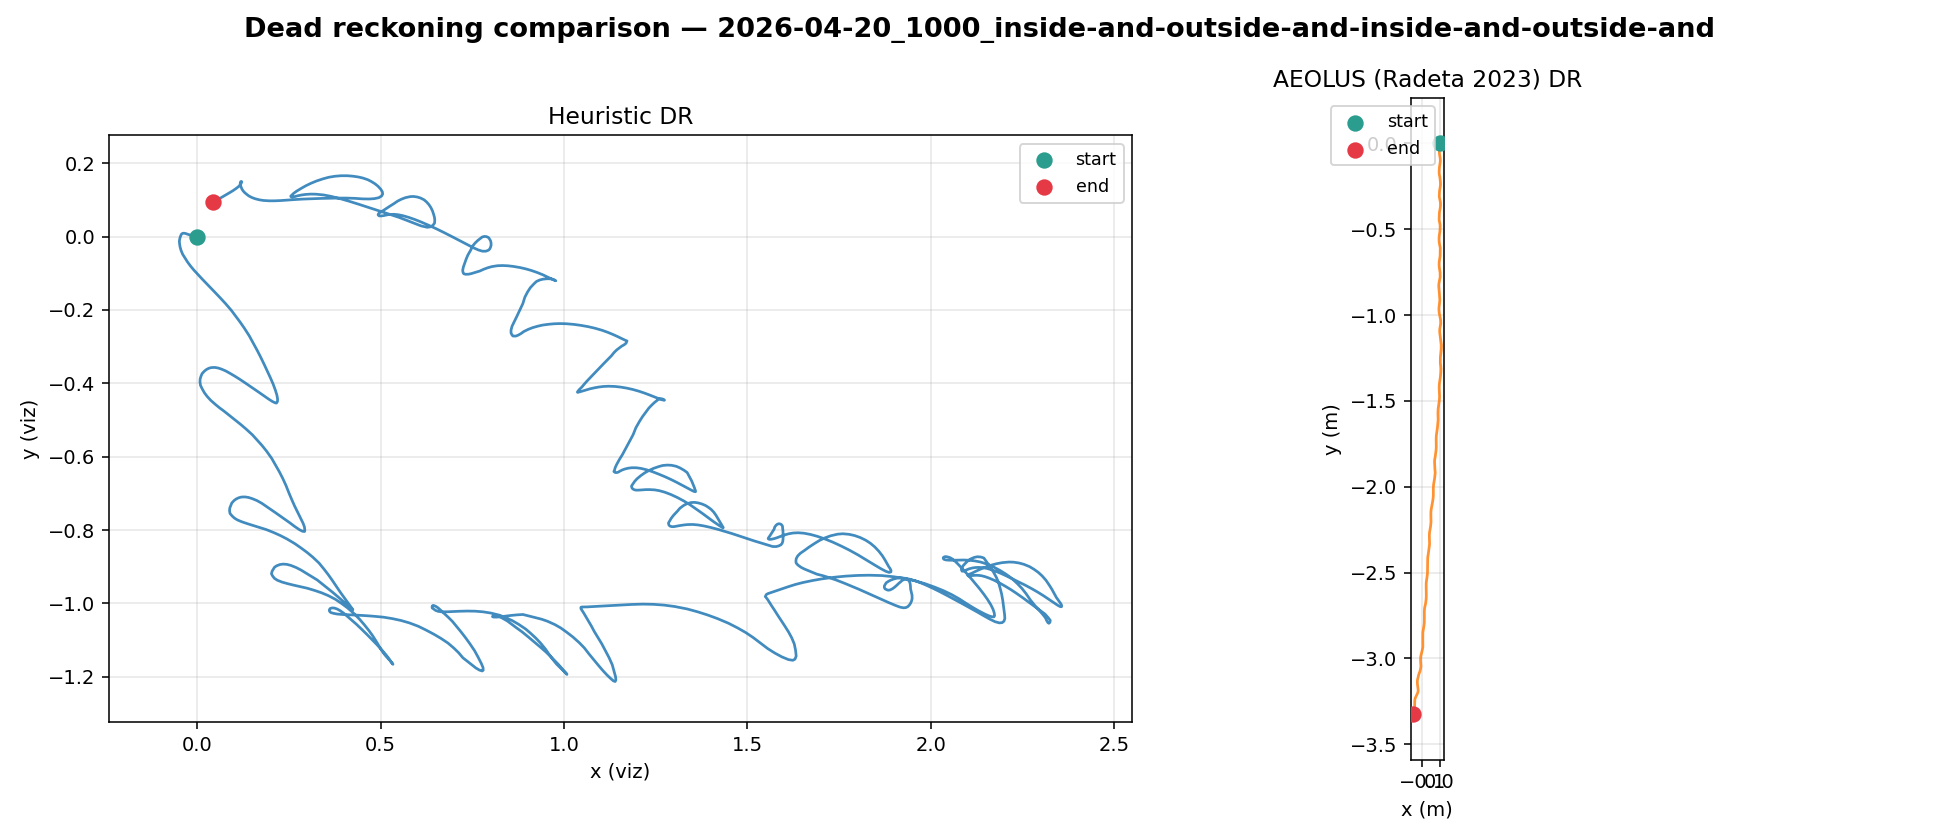
\includegraphics[width=\linewidth]{2026-04-20_1000_inside-and-outside-and-inside-and-outside-and_dr-compare.png}
\caption{Inside-outside brushing session. The heuristic shows a curving sweep
back to roughly the origin; AEOLUS collapses to an almost-1D drift along
$y$ (note the AEOLUS $x$-range is so small that the panel is nearly empty).}
\label{fig:io}
\end{figure}

\begin{figure}[h]
\centering
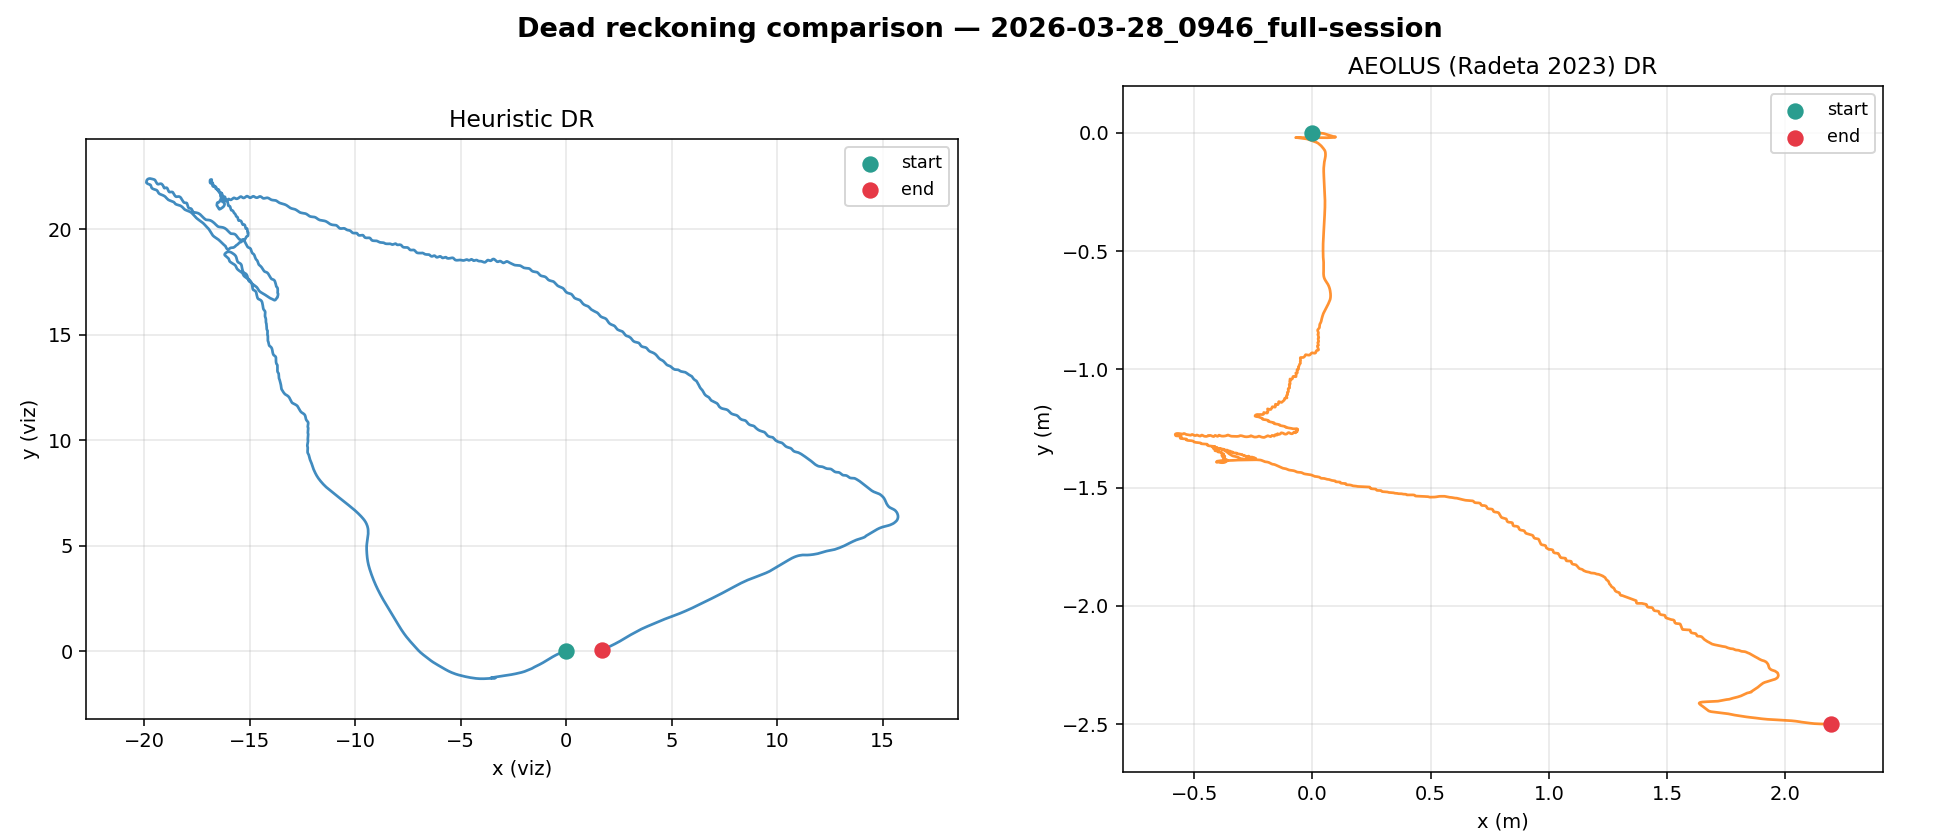
\includegraphics[width=\linewidth]{2026-03-28_0946_full-session_dr-compare.png}
\caption{Full freeform brushing session. Here both methods produce a path
with non-trivial topology: a wide tour through the upper half (heuristic) and
a meander through the right half (AEOLUS), both returning toward the origin.}
\label{fig:full}
\end{figure}

\section{Discussion}
\label{sec:discussion}

\paragraph{Why AEOLUS drifts so heavily on simple motion clips.}
The ZVU step in Algorithm~\ref{alg:aeolus-zvu} only fires when
$|a_{\mathrm{lin}}| < 0.05$\,m/s$^2$, i.e.\ essentially never during active
brushing: the ring is in constant low-grade motion. Without the ZVU
intervening, the literal ``replacement'' velocity assignment $v \gets a \cdot
\Delta t$ produces a small but non-zero step whose sign is set by the
\emph{current} linear acceleration. Because brushing motion is roughly
periodic but not perfectly symmetric, even a small DC bias in
$\mathbf{a}_{\mathrm{lin}}$ accumulates monotonically over the session. This
is exactly the path-versus-end signature we see in the left/right and up/down
rows of Table~\ref{tab:summary}: AEOLUS' end-displacement is 73\%--99\% of
its path length, meaning almost everything that's integrated stays
integrated.

\paragraph{Why the heuristic looks ``right'' on those same clips.}
The heuristic resets state at the window boundary and subtracts the
per-window mean accelerometer reading. Because the brushing motion is
oscillatory within a window, this mean is a good proxy for the gravity
projection and any drift-inducing DC bias, so the integrator sees a
zero-mean signal and produces a zero-mean trajectory. This is what gives
the heuristic its 0.7--1.5\% end/path ratios across all single-motion
sessions: each window's contribution is bounded and centred. The cost is
non-metric output: the path length 109.7 ``viz units'' on the full session
is not in metres or any other physical unit, and the four constants in
Algorithm~\ref{alg:heuristic} are tuned for the brushing motion specifically.

\paragraph{Convention assumption.}
The Earth-frame gravity removal in Equation~\ref{eq:gravity} assumes the ring
reports Euler angles in the ZYX intrinsic Tait-Bryan convention. If the
device uses a different rotation order or sign convention, gravity is not
fully removed and a residual constant acceleration appears in
$\mathbf{a}_{\mathrm{lin}}$. Sanity check from the idle calibration: with
mean roll $\approx -134.1^\circ$ and mean pitch $\approx 31.4^\circ$, the
expected $\mathbf{g}_b$ under ZYX is approximately $(-5.11, -6.02, -5.83)$,
while the measured idle mean is $(5.09, -2.87, 7.82)$. The magnitudes are
close (both $\approx 9.8$\,m/s$^2$) but the directions do not match: the
device's convention is not vanilla ZYX. Tuning candidates if the residual
matters for downstream use: try YXZ/ZXY orderings, or flip the sign of roll
and pitch before constructing the gravity vector.

\paragraph{Faithfulness versus realism.}
We followed the printed Algorithm 1 of \cite{radeta2023} literally: the else
branch is a replacement, $v \gets a \cdot \Delta t$, not an accumulation
$v \gets v + a \cdot \Delta t$. The replacement form has the effect of
high-passing the velocity signal: it forgets prior acceleration entirely the
moment motion resumes, which dampens the explosive drift that the
double-integration form would produce but also throws away the integrating
behaviour that is the whole point of dead reckoning. We believe this is a
typo in the paper; under the accumulation reading the AEOLUS paths would be
larger and more drifty (the paper's own results indicate $5\%$ displacement
error over tens of metres of travel, which is consistent with accumulation
plus working ZVU). Swapping to accumulation is a one-line change in
\texttt{core.py} for users who want to A/B both readings.

\paragraph{Equation 9 as a 2D oddity.}
Equation 9 of \cite{radeta2023} reads $x_i = \Delta x \cos\theta + x_{i-1}$
and $y_i = \Delta y \sin\theta + y_{i-1}$. This is not the usual
heading-rotation formula (which would mix $\Delta x$ and $\Delta y$ through
both $\cos$ and $\sin$). At $\theta = 0$ this becomes $x_i = \Delta x +
x_{i-1}$, $y_i = y_{i-1}$, dropping the $\Delta y$ contribution entirely. We
implement equation 9 as printed; a reader who treats $\Delta x = \Delta y =
\Delta$ (the scalar magnitude of the step) recovers the standard PDR
formula. Both interpretations are easy to swap at one line in the
\texttt{estimate\_dead\_reckoning\_aeolus} function.

\section{Conclusions}

For the smart-ring brushing visualisation, the in-house heuristic is the
right tool: it captures repetitive in-mouth motion cleanly, its output
already lives in viz coordinates, and its four free parameters are
explicitly fit to the cursor-placement objective. The AEOLUS port has value
mainly as a sanity check and as a starting point for a metric trajectory
estimate. With the faithful Algorithm 1 transcription, AEOLUS systematically
under-estimates oscillation amplitude. Restoring the standard accumulation
form, sharpening the ZVU threshold for ring-specific motion, and verifying
the Euler-angle convention would all push the AEOLUS path closer to a
metric ground truth, at which point the comparison shifts from ``which one
looks more reasonable'' to ``which one predicts brushed area more
accurately.'' Both directions are easy follow-ups from the code already in
place.

\begin{thebibliography}{1}

\bibitem{radeta2023}
Marko Radeta, Claudio Rodrigues, Francisco Silva, Pedro Abreu, Jo\~ao Pestana,
Ngoc Thi Nguyen, Agustin Zuniga, Huber Flores, Petteri Nurmi.
\newblock Lost in the Deep? Performance Evaluation of Dead Reckoning Techniques
in Underwater Environments.
\newblock \emph{Proceedings of the ACM on Interactive, Mobile, Wearable and
Ubiquitous Technologies}, 7(2), Article 73, June 2023.
\newblock \href{https://doi.org/10.1145/3596245}{doi:10.1145/3596245}.

\end{thebibliography}

\end{document}
